\begin{figure*}[t]
	\centering
  %https://docs.google.com/drawings/d/1hXY1fwvREalsi9JpvJYvry8uEycz2XQH5jfAyFuhyJs/edit
  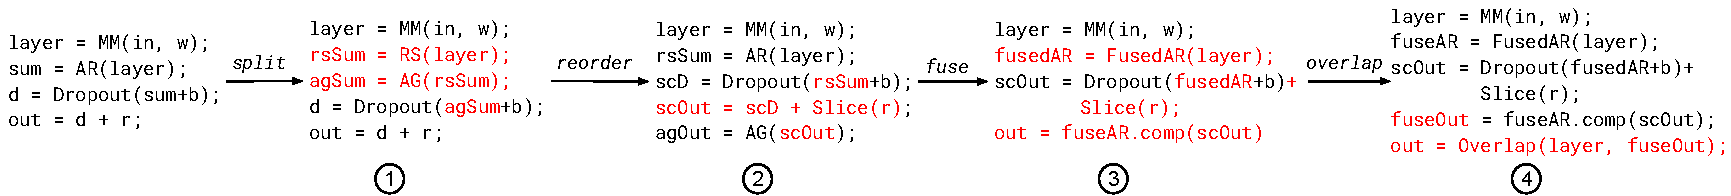
\includegraphics[width=\linewidth]{figures/coconet-example.pdf}
  \caption{\tool programs produced by performing transformations on the program of Figure~\ref{fig:traditional-mp}. Each schedule can be represented as a standalone program. Lines in \textcolor{red}{red} highlights changes at a step. (\texttt{AR}: AllReduce, \texttt{AG}: AllGather, and \texttt{RS}: ReduceScatter)
%  	to the program produced after applying the transformation.
  	\label{fig:mp-schedules}}
    \vspace{-1em}
\end{figure*}

\section{\tool Transformations}
\label{sec:schedule}
\tool provides four semantics preserving \emph{transformations} to optimize a program written in the DSL.
All transformations are valid based on rules described in the sections below. 
\tool automatically checks the validity of each transformation based on these rules and throws an error for  an invalid transformation.

We call an order of transformations a \emph{schedule}.
A user can manually specify the schedule to optimize the program.
Additionally, a user can invoke the autotuner to automatically find the best performing schedule for the given problem sizes and the underlying architecture.
Below we present each transformation by applying them on the program from Figure~\ref{fig:traditional-mp} and show equivalent \tool{} programs generated after applying each transformation in Figure~\ref{fig:mp-schedules}.

\subsection{Splitting Communication}
The \texttt{split} transformation breaks a collective communication operation into two communication operations.
One of the two split policies supported by \tool is

\textbf{AllReduce Split RS-AG} splits an \allreduce into a \reducescatter to produce a \sliced tensor and an \allgather on the \sliced tensor to return a \replicated tensor.

% \textbf{AllReduce Split B-R} splits an \allreduce into a \reduce to produce a tensor on user specified root rank and then \broadcast this tensor to all ranks in \WORLD.

\spara{Running Example} The \allreduce in Figure~\ref{fig:traditional-mp} is split into \texttt{rsSum} that does a \reducescatter on \texttt{layer} and \texttt{agSum} that does an \allgather on \texttt{rsSum}.
{
\small
\begin{lstlisting}[language=DSL,numbers=none]
(rsSum, agSum) = split(layer, ARSplitRSAG);
\end{lstlisting}
}

The program \circled{1} of Figure~\ref{fig:mp-schedules} is the implementation of this schedule where the input to Dropout is replaced by \texttt{agSum}.

\spara{\textit{Validity}} Since an \allreduce can always be split to a \reducescatter and an \allgather, this transformation is always valid.

\begin{figure}[t]
	\centering
	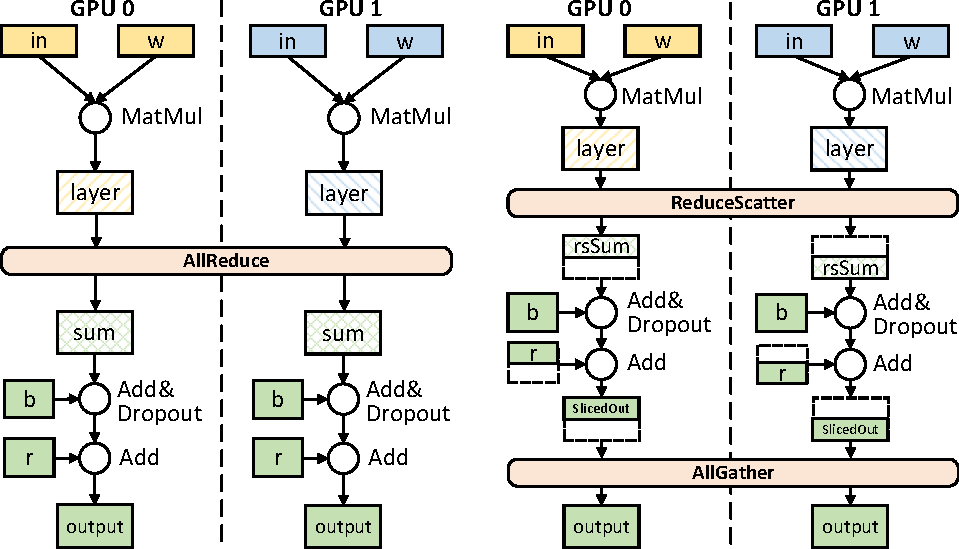
\includegraphics[width=.9\linewidth]{figures/reduceScatter}
%	\caption{Example of parallel Self-Attention layer on two GPUs using AllReduce (on left) and using ReduceScatter + AllGather (on right).}
	\caption{Equivalent programs (from Figure~\ref{fig:traditional-mp}) using AllReduce (on left) or using ReduceScatter + AllGather (on right).}
	\label{fig:model-parallel-using-reducescatter}
\end{figure}

\subsection{Reordering Operations}
The \texttt{reorder} transformation swaps operations with an \allgather or a \broadcast in the DFG of a program.
We explain this transformation for \allgather below: 

\textbf{AllGather Reorder} reorders an \allgather with communication and computation operations. 
This transformation changes the layout of the operations, the input and output of operations, and the input and output of the \allgather.
We explain this transformation below using the running example.

% \textbf{Broadcast Reorder} is similar to \allgather reorder except that it requires the user to specify a root rank.

\spara{Running Example}
In Figure~\ref{fig:mp-schedules}, applying the \texttt{reorder} transformation changes the program \circled{1} to \circled{2} by reordering \allgather (\texttt{agSum}) with computations \texttt{d} and \texttt{out}.
The reorder transformation replaces these operations in the DFG with three new operations: \texttt{scD} and \texttt{scOut},
both of which performs sliced computations, and \texttt{agOut}, which gathers the final result of computations.
{
  \small
\begin{lstlisting}[language=DSL,numbers=none]
(scD, scOut, agOut) = reorder(d, out, agSum);
\end{lstlisting}
}
The new sliced computations perform the same operations as original computations with two differences: (i) the output of \allgather used in the computation is replaced by the input of \allgather, and (ii) since the input of \allgather is sliced, 
all tensors input to the computations are also sliced along the same dimension as the input of \allgather.
After reorder, \texttt{scD} performs the same computation as \texttt{d} but \texttt{scD} takes \texttt{rsSum} and \texttt{Slice(r)} as input.
Therefore, the layout of \texttt{scOut} is also sliced while the computation is same as \texttt{out}.
Furthermore, the new \allgather is performed on the outputs of the computations, for example, 
after reorder, the \allgather (\texttt{agOut}) is performed on \texttt{scOut}.
Figure~\ref{fig:model-parallel-using-reducescatter} shows the workflow of this schedule.
% Here the input to Dropout is now the output of \reducescatter (\texttt{rsSum}) and computations are performed on slice of residual (\texttt{r}) to produce a sliced output.
% Then, \allgather collects the sliced output to obtain a replicated output.
% The next section describes fusion of communication and computation. 

\spara{\textit{Validity}} The \texttt{reorder} transformation is valid only if operations being reordered with an \allgather can be sliced along the dimension the \allgather is performed.
The rules of slicing an operation depend on the type of operation and the dimensions of inputs to the operations.
For example, \texttt{d} and \texttt{out} can be sliced because the computations have the same dimensions as \texttt{agOut}.
Section~\ref{sec:opt-workloads} shows how P2P Send can be reordered with an \allgather.
% A MatMul can be sliced in the rows or columns dimension of the output matrix but not in the reduction dimension.

\subsection{Fusing Operations}
\label{sec:sched:fusion}

Fusing multiple computations is a common technique used by existing compilers~\cite{tvm18,distributed-halide,fireiron,polymage-gpu,halide}.
\tool extends this concept to fuse multiple computations and communications in a single operation and provides this capability using the \texttt{fuse} transformation.
Below we explain two fuse policies supported by \tool:

\textbf{Computation Fuse} fuses a series of computations in a single operation that performs all these operations.

\textbf{AllReduce Fuse} fuses a series of \reducescatter, sliced computations, and \allgather operations in a single Fused\allreduce that performs all these operations.

\spara{Running Example}
We can fuse \reducescatter (\texttt{rsSum}), computations (\texttt{scD} and \texttt{scOut}), and \allgather (\texttt{agOut}) in program \circled{2} of Figure~\ref{fig:mp-schedules} into a Fused\allreduce to obtain program \circled{3}.
{
\small
\begin{lstlisting}[language=DSL,numbers=none]
fuseAR = fuse(rsSum, scOut, agOut, ARFuse);
\end{lstlisting}
}
The \texttt{comp} method of \texttt{fusedAR} specifies the computation to be fused with Fused\allreduce and returned \texttt{out} is the output.

\spara{\textit{Validity}} Fusing multiple operations into one operation is valid only if the dependencies in the DFG after fusion are preserved.

\subsection{Overlapping Operations}
\tool provides the \texttt{overlap} transformation to overlap a series of producer-consumer operations to utilize multiple resources of hardware simultaneously.
% One use case of this transformation is to overlap computation and communication operations.
% It takes two or more operations as input and returns a single operation.

\spara{Running Example} 
In the program \circled{3} of Figure~\ref{fig:mp-schedules} we overlap the matrix multiplication (\texttt{layer}) with Fused\allreduce (\texttt{fuseAR}) to obtain program in \circled{5}.
{
\small
\begin{lstlisting}[language=DSL,numbers=none]
layerWithAR = overlap(layer, fusedAR);
\end{lstlisting}
}

\spara{\textit{Validity}} Overlapping multiple operations is valid only when all operations have a producer-consumer relationship between them.

% Operation returned by \texttt{Overlap} is the final output of the program.

\subsection{Automatic Exploration of Schedules}
\tool provides an \emph{autotuner} to automatically explore the space of all schedules of a program and return the schedule that provides the best performance for the underlying architecture and input sizes.
First, the autotuner fuses all pointwise computations up to a pre-defined threshold to decrease the search space and then exhaustively explores the schedule space in a breadth first search manner.
Finally, the autotuner generates code for all schedules in its search space, executes all programs, and returns the schedule with minimum execution time.
Table~\ref{tab:loc-autotuner-time} shows that the autotuner takes only a few seconds to explore the schedule space for all workloads.

\begin{figure}
  \small
  \centering
% Scalar lr(FP32), beta1(FP32), beta2(FP32);|\label{line:adam:scalars}|
% Tensor g(FP32, WORLD_SZ, SIZE, Sliced); |\label{line:adam:inputensor-begin}||\label{line:adam:continuous-tensor}|
% Tensor p(FP32, WORLD_SZ, SIZE, Replicated);
% Tensor m(FP32, WORLD_SZ, SIZE, Replicated);
% Tensor v(FP32, WORLD_SZ, SIZE, Replicated);|\label{line:adam:inputensor-end}| 
  \begin{subfigure}[t]{\columnwidth}
\begin{lstlisting}[language=DSL, numbers=left]
Var avg = AllReduce("+", g); |\label{line:adam:avg}|
Var m_ = Update(m, (m*beta1+(1-beta1)*avg));|\label{line:adam:pointwise-begin}||\label{line:update:m}|
Var v_ = Update(v, (v*beta2+(1-beta1)*avg*avg));|\label{line:update:v}|
Var m1 = m_/(1-Pow(beta1, t));
Var v1 = v_/(1-Pow(beta2, t));
Var p_ = Update(p, (p - lr * m1/(Sqrt(v1))));|\label{line:adam:pointwise-end}|

Execute adam({g,p,v,m,lr}, {p_});
\end{lstlisting}
\caption{Traditional implementation where 
               tensors \texttt{g} is local to each rank and \texttt{p},\texttt{m}, and \texttt{v} are replicated on all ranks.}
\label{fig:traditional-adam}
\end{subfigure}
\par\bigskip % Do not remove this. Without this there is no space between caption of above figure and the next figure. WEIRD bug. Never saw this in subfigure.
\begin{subfigure}[b]{\columnwidth}
\begin{lstlisting}[language=DSL, numbers=left]
comps = fuse(m_, v_, m1, v1, p_, 
             ComputationFuse);|\label{line:adam-schedule:fuse-comp}|
(rsG, agG) = split(avg, ARSplitRSAG); |\label{line:adam-schedule:split}|
(scComp, agP, agM, agV) = reorder(agG, comps, 
                                  AGReorder);|\label{line:adam-schedule:reorder}|  
asSlice(m); asSlice(v); dead(agM); dead(agV); |\label{line:adam-schedule:slice-m-v}| |\label{line:adam-schedule:remove-m-v-allgather}|
fuseAR = fuse(rsG, scComp, agP, AllReduceFuse);|\label{line:adam-schedule:fuse-allreduce}|
\end{lstlisting}
\caption{An Optimized Schedule. Tensors \texttt{g} is local, \texttt{p} is replicated on all ranks, while 
\texttt{m} and \texttt{v} are sliced among all ranks.}
\label{fig:adam-schedule}
\end{subfigure}
% Scalar lr(FP32), beta1(FP32), beta2(FP32);|\label{line:adam:scalars}|
% Tensor g(FP32, WORLD_SZ, SIZE, Sliced); |\label{line:adam:inputensor-begin}||\label{line:adam:continuous-tensor}|
% Tensor p(FP32, SIZE, Replicated);
% Tensor m(FP32, SIZE, Sliced);
% Tensor v(FP32, SIZE, Sliced);|\label{line:adam:inputensor-end}| 
% \hfill{}
% \begin{subfigure}{0.32\textwidth}
%   \begin{lstlisting}[language=DSL, numbers=left]
% avg = FusedAllReduce("+", g); |\label{line:adam:avg}|
% scP_ = p.update(p - scDiff);
% p_ = fuseAR.comp(scP_);

% adam({g,p,v,m,lr}, {p_});
%   \end{lstlisting}
% \caption{Equivalent \tool implementation after applying the schedule. 
% Tensors \texttt{g} and \texttt{p} are replicated on all ranks, while 
% \texttt{m} and \texttt{v} are sliced among all ranks. \texttt{scDiff}
% represents the sliced \texttt{diff}. \label{fig:optimized-adam}}
% \end{subfigure}
  \caption{Optimizing parameter update using Adam in \tool. 
  The implementation takes four input tensors: parameters (\texttt{p}), gradients (\texttt{g}),
  momentum (\texttt{m}), and velocity (\texttt{v}).
  \label{fig:optimizing-adam}}
  \end{figure}

\section{Distributed Workloads in \tool}
\label{sec:opt-workloads}
We additionally optimized two distributed machine learning workloads using \tool: (i) parameter update using Adam~\cite{adam}, and (ii) point-to-point communication in pipeline parallelism.

\spara{Adam in Data Parallel Training}: Figure~\ref{fig:traditional-adam} shows the traditional implementation of parameter update using Adam.
First, all ranks average the gradients using \allreduce and then perform computations to update the optimizer state and model parameters.
\texttt{Update} updates the values of a tensor and reflects the new values in that position in the DFG (lines~\ref{line:update:m}--\ref{line:update:v}).
Figure~\ref{fig:adam-schedule} presents a schedule that optimizes this by distributing the computation on all ranks in a single kernel.
Line~\ref{line:adam-schedule:fuse-comp} fuses all computations in \texttt{comps}.
Line~\ref{line:adam-schedule:split} splits the \allreduce into a \reducescatter and an \allgather, such that computations take output of \allgather (\texttt{agG}) as input.
Line~\ref{line:adam-schedule:reorder} reorders \allgather with computations, such that,
each rank performs computations on a slice of tensors.
% \allgather operations are returned for parameters and optimizer state.
Line~\ref{line:adam-schedule:slice-m-v} slices optimizer states on all ranks to decrease memory usage and removes corresponding \allgather.
Finally, line~\ref{line:adam-schedule:fuse-allreduce} fuses all operations in a single kernel.

\begin{figure}[t]
  \begin{subfigure}{\columnwidth}
  \centering
  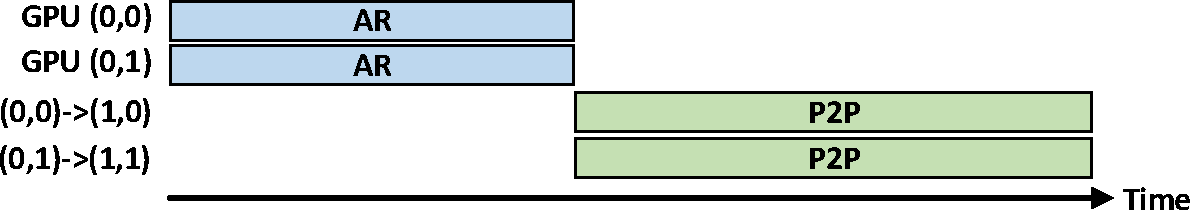
\includegraphics[width=.85\linewidth]{figures/pipeline-p2p-fusion-1.pdf}  
  \caption{In Megatron-LM each GPU sends redundant data. \label{fig:p2p-fusion-1}}
\end{subfigure}
\par\bigskip % Do not remove this. Without this there is no space between caption of above figure and the next figure. WEIRD bug. Never saw this in subfigure.
\begin{subfigure}{\columnwidth}
  \centering
  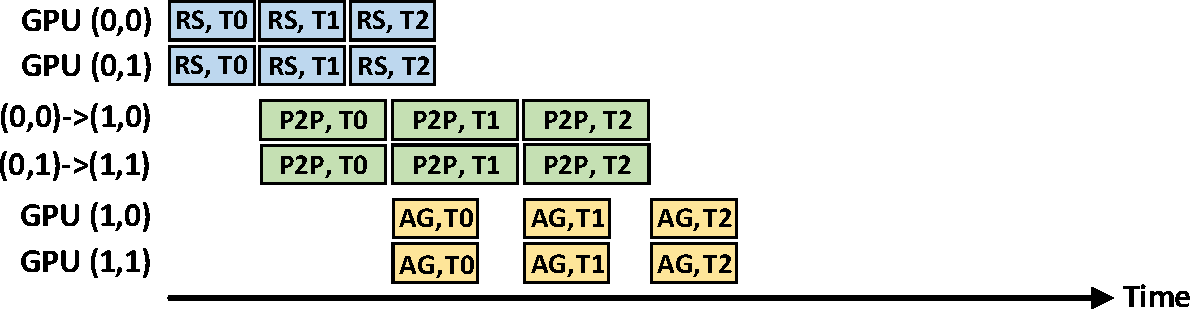
\includegraphics[width=.85\linewidth]{figures/pipeline-p2p-fusion-3.pdf} 
  \caption{Communication operations can be overlapped at the granularity of each 
  \emph{communication buffer tile} of data in single kernel 
  call.\label{fig:p2p-fusion-3}}
\end{subfigure}
  \caption{Two different schedules of pipeline parallelism.
\label{fig:P2Ptimeline}}
\end{figure}

\spara{Point-to-Point Communication in Pipeline Parallelism}: 
Figure~\ref{fig:p2p-fusion-1} shows a scenario of pipeline parallelism in Megatron-LM
with two transformer layers assigned to two groups each with two ranks. 
Rank $i$ in group $j$ is shown by $(j,i)$.
Each group uses model parallelism within its transformer layer.
Pipeline parallelism in Megatron-LM works as follows.
First, all ranks in the first group reduce their input using 
\allreduce to get replicated output.
Then each rank performs pointwise computations over the replicated output.
Finally, the first group sends the result of computations to the corresponding rank in the
second group using point-to-point (P2P) sends. (Line~\ref{line:p2p:comp2} in Figure~\ref{fig:traditional-p2p} shows these computations but are omitted in Figure~\ref{fig:P2Ptimeline} for simplicity). Since the output of \allreduce in 
Figure~\ref{fig:p2p-fusion-1} is replicated, redundant data is sent using P2P.
We can avoid this redundant communication by splitting
the \allreduce to \reducescatter and \allgather and reordering the P2Ps with the
\allgather. 
Hence, the inter-group communication is reduced by 
the group size.
We can further optimize by overlapping all communication operations. 
Figure~\ref{fig:p2p-fusion-3} shows that if the 
buffers are split into multiple tiles (\texttt{T0}--\texttt{T2} in the figure), 
intra-group and inter-group communications can be overlapped.
%  to further reduce the communication time.

% Figure~\ref{fig:optimizing-p2p} shows how to do these 
% optimizations with \tool. 
Figure~\ref{fig:traditional-p2p} is the original program, 
while Figure~\ref{fig:p2p-schedule} optimizes it by applying transformations.
Line~\ref{line:p2p:fuse-send} fuses the P2P 
send with computations.
Line~\ref{line:p2p:split} splits the \allreduce and reorders the returned \allgather with the fused P2P send at Line~\ref{line:p2p:reorder}.
Hence, P2P send and computations are performed 
on only a slice of data on the next group where the \allgather is also performed.
Finally, all three new operations get overlapped in Line~\ref{line:p2p:fuseAR}.
% This overlapping can only be achieved by generating custom communication and computation kernels.
%Figure~\ref{fig:traditional-p2p} shows the implementation of pipeline parallelism in Megatron-LM.
%Here one Transformer layer is assigned to a group of consecutive ranks, such that each group uses model parallelism for the Transformer layer.
%First all ranks in a group perform reduces their input (\texttt{in}) using \allreduce to obtain a replicated output.
%Each rank in the group sends the output to same rank of next group using point-to-point (P2P) communication, over which several pointwise computations are done.
%Figure~\ref{fig:p2p-schedule} optimizes the program by avoiding send of redundant replicated output. 
%Lines~\ref{line:p2p:fuse-comp}--\ref{line:p2p:fuse-send} fuses the P2P send with computations.
%At line~\ref{line:p2p:reorder} \allreduce is split and the returned \allgather is reordered with fused send, so that, both P2P send and computations are performed on only a slice of data on the next group and the \allgather is also performed on the next group.
%Finally, all three new operations can be overlapped because \reducescatter and \allgather are performed in different groups and P2P send uses interconnect between the groups.

\begin{figure}[!t]
	\small
	\begin{subfigure}{\columnwidth}
		\begin{lstlisting}[language=DSL, numbers=left]
Var sum = AllReduce("+", in);
Var send = Dropout(recv+b,0.1) + r;|\label{line:p2p:comp1}||\label{line:p2p:comp2}|
Var output = Send(send, 
                  GroupRank(GROUP+1, RANK));

Execute transformer({in}, {output});
		\end{lstlisting}
		\caption{Traditional implementation. Each rank of a group sends same data to next group.}
		\label{fig:traditional-p2p}
	\end{subfigure}
	\par\bigskip % Do not remove this. Without this there is no space between caption of above figure and the next figure. WEIRD bug. Never saw this in subfigure.
	\begin{subfigure}{\columnwidth}
		\begin{lstlisting}[language=DSL, numbers=left]
fuseSend = fuse(send, output, SendFuse);|\label{line:p2p:fuse-send}|
(rsSum, agSum) = split(sum, ARSplitRSAG); |\label{line:p2p:split}|
(scSend, agOut) = reorder(fuseSend, agSum, 
                          AGReorder); |\label{line:p2p:reorder}|
overlapOut = overlap(rsSum, scSend, agOut); |\label{line:p2p:fuseAR}|
		\end{lstlisting}
		\caption{An Optimized Schedule. Each rank sends only a slice of data to ranks in next group and all operations are overlapped.}
		\label{fig:p2p-schedule}
	\end{subfigure}
	\caption{Optimizing pipeline parallelism of Megatron-LM. Input tensors: layer output \texttt{in}, bias \texttt{b}, and residual \texttt{r}. \label{fig:optimizing-p2p}}
\end{figure}


\iffalse

\begin{figure*}[t]
    \small
\begin{subfigure}{0.49\textwidth}
    \begin{lstlisting}[language=DSL]
    Variable lr(Float);
    Variable m(Float);
    Tensor g(Float, SIZE, GPUs);
    Tensor p(Float, SIZE, GPUs);
    Tensor v(Float, SIZE, GPUs);
    
    Stage sum = AllReduce("+", g);
    Stage v_ = m * v + sum/GPUs;
    Stage p_ = p - lr * v_;
    
    Pipeline pipeline({g, p, m, lr}, {v}, {p_});
\end{lstlisting}
\caption{Optimizing  SGD in \tool }
    \label{fig:traditional-sgd}
\end{subfigure}

\begin{subfigure}{0.45\textwidth}
\begin{lstlisting}[language=DSL]     
        Stage sumRS;
        Stage sumAG;
        pipeline.split(sum, &sumRS, &sumAG, 
                       ReduceScatterAllGather); 
\end{lstlisting}
\caption{}
\end{subfigure}
\begin{subfigure}{0.45\textwidth}
        \begin{lstlisting}[language=DSL]     
                sumRS = ReduceScatter(g); 
                sumAG = AllGather(sumRS)
                //Replace all references of 
                //sum with sumAG
        \end{lstlisting}
        \caption{}
\end{subfigure}

\begin{subfigure}{0.45\textwidth}
\begin{lstlisting}[language=DSL]     
        Stage v1_, vAG;
        pipeline.reorder(v_, sumAG, v1_, vAG); 
\end{lstlisting}
\caption{}
\end{subfigure}
\begin{subfigure}{0.45\textwidth}
        \begin{lstlisting}[language=DSL]     
                v1_ = m * slice(v) + sumRS/GPUs; 
                vAG = AllGather(v1_);
                p_ = p - lr * vAG;
        \end{lstlisting}
        \caption{}
\end{subfigure}

\begin{subfigure}{0.45\textwidth}
\begin{lstlisting}[language=DSL]     
        Stage p1_, pAG;
        pipeline.reorder(vAG, p_, p1_, pAG); 
        pipeline.asSlice(v); 
        pipeline.fuse({sumRS, v1_, p1_, pAG}, 
                      AllReduce); 
        pipeline.storeAt({p_, p},{v_, v});
\end{lstlisting}
\caption{}
\end{subfigure}
\begin{subfigure}{0.45\textwidth}
\begin{lstlisting}[language=DSL]     
        v1_ = m * slice(v) + sumRS/GPUs; 
        pAG_ = slice(p) - lr * v1_; 
        p1_ = AllGather(pAG_);
\end{lstlisting}
\caption{}
\end{subfigure}

\begin{subfigure}{0.45\textwidth}
\begin{lstlisting}[language=DSL]     
        pipeline.asSlice(v); 
        pipeline.fuse({sumRS, v1_, p1_, pAG}, 
                        AllReduce); 
        pipeline.storeAt({p1_, p},{v1_, v});
\end{lstlisting}
\caption{}
\end{subfigure}
\caption{SGD with momentum}
\end{figure*}



\begin{figure*}[t]
    \small
\begin{subfigure}{0.49\textwidth}
    \begin{lstlisting}[language=DSL]
    Variable lr(Float);
    Variable m(Float);
    Tensor g(Float, SIZE, GPUs);
    Tensor p(Float, SIZE, GPUs);
    Tensor v(Float, SIZE, GPUs);
    Tensor m(Float, SIZE, GPUs);
    
    Stage sum = AllReduce("+", g);
    Stage m_ = beta1 * m + (1-beta1)*sum;
    Stage v_ = beta2 * v + (1-beta2)*(sum*sum);
    Stage p_ = p - lr * m_/(1-beta1)/(sqrt(v_/(1-beta2)));
    
    Pipeline pipeline({g, p, m, lr}, {v}, {p_});
\end{lstlisting}
\caption{Optimizing  Adam in \tool }
    \label{fig:traditional-sgd}
\end{subfigure}

\begin{subfigure}{0.45\textwidth}
\begin{lstlisting}[language=DSL]     
        Stage sumRS;
        Stage sumAG;
        pipeline.split(sum, &sumRS, &sumAG, 
                       ReduceScatterAllGather); 
\end{lstlisting}
\caption{}
\end{subfigure}
\begin{subfigure}{0.45\textwidth}
        \begin{lstlisting}[language=DSL]     
                sumRS = ReduceScatter(g); 
                sumAG = AllGather(sumRS)
                //Replace all references of 
                //sum with sumAG
        \end{lstlisting}
        \caption{}
\end{subfigure}

\begin{subfigure}{0.45\textwidth}
\begin{lstlisting}[language=DSL]    
        Stage mv;
        pipeline.fuse({m_,v_}, mv) ;
        Stage mv_, mvAG;
        pipeline.reorder(mv_, sumAG, mv1_, mvAG); 
\end{lstlisting}
\caption{}
\end{subfigure}
\begin{subfigure}{0.45\textwidth}
        \begin{lstlisting}[language=DSL]     
                Stage m_ = beta1 * slice(m) + (1-beta1)*sumRS;
                Stage v_ = beta2 * slice(v) + (1-beta2)*(sumRS*sumRS);
                vAG = AllGather(v1_);
                mAG = AllGather(m1_);
                p_ = p - lr * f(mAG, vAG);
        \end{lstlisting}
        \caption{}
\end{subfigure}

\begin{subfigure}{0.45\textwidth}
\begin{lstlisting}[language=DSL]     
        Stage p1_, pAG;
        pipeline.reorder(mvAG, p_, p1_, pAG); 
        pipeline.asSlice(v); 
        pipeline.asSlice(m); 
        
\end{lstlisting}
\caption{}
\end{subfigure}
\begin{subfigure}{0.45\textwidth}
\begin{lstlisting}[language=DSL]     
        v1_ = m * slice(v) + sumRS/GPUs; 
        pAG_ = slice(p) - lr * v1_; 
        p1_ = AllGather(pAG_);
\end{lstlisting}
\caption{}
\end{subfigure}

\begin{subfigure}{0.45\textwidth}
\begin{lstlisting}[language=DSL]     
        pipeline.asSlice(v); 
        pipeline.fuse({sumRS, v1_, p1_, pAG}, 
                        AllReduce); 
        pipeline.storeAt({p1_, p},{v1_, v});
\end{lstlisting}
\caption{}
\end{subfigure}
\caption{Adam}
\end{figure*}


\begin{figure*}[t]
        \small
\begin{subfigure}{0.49\textwidth}
        \begin{lstlisting}[language=DSL]
        Variable lr(Float);
        Variable m(Float);
        Tensor g(Float, SIZE, GPUs);
        Tensor p(Float, SIZE, GPUs);
        Tensor v(Float, SIZE, GPUs);
        Tensor m(Float, SIZE, GPUs);
        
        Stage sum = AllReduce("+", g);
        Stage m_ = beta1 * m + (1-beta1)*sum;
        Stage v_ = beta2 * v + (1-beta2)*(sum*sum);

        Stage r1 = Reduce("+", p * p);
        Stage p_upd = m_ / sqrt(v_ + eps) + lambda * p
        Stage r2 = Reduce("+", p_upd * p_upd)

        Stage p_ = p - r1/r2*lr* p_upd
        
        Pipeline pipeline({g, p, m, lr}, {v}, {p_});
    \end{lstlisting}
\end{subfigure}
\caption{LAMB}

\begin{subfigure}{0.49\textwidth}
        \begin{lstlisting}[language=DSL]
        Variable lr(Float);
        Variable m(Float);
        Tensor g(Float, SIZE, GPUs);
        Tensor p(Float, SIZE, GPUs);
        Tensor v(Float, SIZE, GPUs);
        Tensor m(Float, SIZE, GPUs);
        Stage p_slc = slice(p)


        Stage sumRS = ReduceScatter("+", g);
        Stage m_slc = beta1 * slice(m) + (1-beta1)*sumRS;
        Stage v_slc = beta2 * slice(v) + (1-beta2)*(sumRS*sumRS);
        Stage p_upd_slc = m_slc / sqrt(v_slc + eps) + lambda * p_slc

        Stage r1 = AllReduce("+", p_slc * p_slc);
        Stage r2 = AllReduce("+", p_upd_slc * p_upd_slc)

        Stage p_slc_ = p_slc - r1/r2*lr* p_upd_slc

        Stage p_ = AllGather(p_slc_)

        Pipeline pipeline({g, p, m, lr}, {v}, {p_});
    \end{lstlisting}
\end{subfigure}

\caption{Optimizing LAMB in \tool }
        \label{fig:lamb}
\end{figure*}

\tool automatically checks validity of each computation based on a set of \emph{validation rules}.
Each validation rule checks the properties of all tensors involved in the computation and assign values to all properties of the output tensor.
Figure~\ref{fig:rules} presents the validation rules for all computations supported by \tool.
In the validation rules the four properties of a tensor (T) are represented as follows: (i) $\type{}$ is the type of elements, 
(ii) $n$ is the number of elements, (iii) $\Locs{}$ is the set of ranks, and (iv) $\alloc{}$ is the allocation type.
Below we explain the validation rules of all computations.

\paragraph{Pointwise Computations} Pointwise computations are valid only if the input tensors have same value of properties and the output tensor will have properties with these values (rules \textsc{E-BinaryOp} and \textsc{E-UnaryOp}).

\paragraph{Communication Collectives} Each computation involving a NCCL Communication Collective computations has a validation rule associated, which follows the semantics of the computation defined in the NCCL documentation~\cite{}.
\allreduce on the input tensor is valid only if the input is a \complete tensor and present on all ranks in the \WORLD (\textsc{E-AllReduce}). After \allreduce, the output tensor has same properties as the input tensor.
Similar to \allreduce, \reducescatter requires same conditions on the input tensor but the output tensor will be equally \sliced among all ranks in \WORLD (rule \textsc{E-ReduceScatter}).
Since \allgather gathers all slices from all ranks and stores these slices in \complete tensors on all ranks, \allgather requires input tensor to be a \sliced tensor stored on all ranks in \WORLD and the output tensor is a \complete (rule \textsc{E-AllGather}).
Slicing a tensor is possible only if it is continuous and the output tensor is stored on all ranks where the input tensor was stored (rule \textsc{E-Scatter}).
So far we have presented the validation rules that can be checked during the compile time.
However, the rules for allocation type for Reduce and Broadcast must be dynamically checked because both requires a particular rank as input, which must be checked at the runtime if it belongs to \WORLD.
These dynamic checks are automatically generated by \tool code generator (discussed in Section~\ref{sec:code-gen}).
\reduce can be called on tensors that are present on all ranks in \WORLD with the target rank in the \WORLD and the output tensor is available on the target rank only (rule \textsc{E-Reduce}).
On the other hand, Broadcast is valid only for \complete tensors and when all nodes in \WORLD will receive the output tensor(rule \textsc{E-Broadcast}).

\paragraph{LoadTensorAtRank}

\paragraph{ReduceTensor} Reducing a single tensor is possible on both \sliced or \complete tensors. However, the tensor must be stored on all ranks in \WORLD (rule \textsc{E-ReduceTensor}).
The output tensor will contain only one element, which will have different value for different ranks.

\paragraph{Cast} According to the validation rule \textsc{E-Cast} the  output tensor has same properties as the input tensor, except the output's element type is the argument of Cast.

\paragraph{Example} We illustrate type checking on \tool code in Figure~\ref{fig:FusedSGD} and Figure~\ref{fig:reduce-scatter-sgd}.
In Figure~\ref{fig:FusedSGD}, \allreduce produces a \complete stage of same size, element type, and on nodes.
Then the computations on lines~\ref{}--\ref{} again produces tensors with same properties. 
In contrast, Figure~\ref{fig:reduce-scatter-sgd} uses a \reducescatter to generate a tensor of size \aj{To be continued}

\begin{figure}[t]
  \small
\begin{subfigure}{\columnwidth}
\(
\begin{array}{@{}l@{}r@{\,}c@{\,}l@{}}
        \textbf{Tensors} & \tensor{}^{[\type{},n,\Locs{}, \alloc{}]}\\
        \text{Element Type} & \type{} & \in & \ldots\\ %\{u8, i8, f16, \cdots,  u64, i64, f64\} \\
        \text{Tensor Size} & n & \in & Z^{+} \\
        \text{Set of all ranks} & WORLD & \subseteq & Z^{+} \\
        \text{Set of Storage Locations} & \Locs{} & \subseteq & WORLD\\
        \text{Allocation Type} & \alloc{} & \in & \{\text{\complete, Sliced}\}\\
        \text{Pointwise Computations} & \texttt{op} & \in &{+, -, *, /, pow}\\
\end{array}
\)
\end{subfigure}

\begin{subfigure}{\columnwidth}
\begin{mathpar}
\inferrule*[Left=E-BinaryOp]
        {\tensor{}_{1}^{[\type{}_1,n_1,\Locs{}_1, \alloc{}_1]} = \texttt{op}(\tensor{}_{2}^{[\type{},n,\Locs{},\alloc{}]}, \tensor{}_{3}^{[\type{},n,\Locs{},\alloc{}]})}
        {\type{}_1 = \type{} \\ n_1 = n \\ \Locs{}_1 = \Locs{} \\ \alloc{}_1 = \alloc{}}\\ %\forall_{\loc{} \in \Locs{}}\forall_{0 \leq i \leq n} \tensor{}_{1}[\loc{}, i] = \texttt{op}(\tensor{}_{2}[\loc{}, i], \tensor{}_{3}[\loc{}, i])
\inferrule*[Left=E-UnaryOp]
        {\tensor{}_{1}^{[\type{}_1,n_1,\Locs{}_1, \alloc{}_1]} = \texttt{op}(\tensor{}_{2}^{[\type{},n,\Locs{},\alloc{}]})}
        {\type{}_1 = \type{} \\ n_1 = n \\ \Locs{}_1 = \Locs{} \\ \alloc{}_1 = \alloc{}}\\ %\forall_{\loc{} \in \Locs{}}\forall_{0 \leq i \leq n} \tensor{}_{1}[\loc{}, i] = \texttt{op}(\tensor{}_{2}[\loc{}, i], \tensor{}_{3}[\loc{}, i])
\inferrule*[Left=E-Slice]
        { {
          \begin{array}{ll}
            \tensor{}_{1}^{[\type{}_1,n_1,\Locs{}_1,\alloc{}_1]} = \texttt{Slice}(\tensor{}^{[\type{},n,\Locs{},\alloc{}]})\\
            \alloc{} = \complete
          \end{array}
        } }
        {
          {
            \begin{array}{ll}
              \type{}_1 = \type{} & n_1 = \frac{n}{|\Locs{}|} \\ 
              \Locs{}_1 = \Locs{} & \alloc{}_1 = \sliced
            \end{array}
          }
        }\\
\inferrule*[Left=E-Cast]
        {\tensor{}_{1}^{[\type{}_1,n_1,\Locs{}_1,\alloc{}_1]} = \texttt{Cast}(\tensor{}^{[\type{},n,\Locs{},\alloc{}]}, \type{}_2)}
        {\type{}_1 = \type{}_2 \\ n_1 = n \\ \Locs{}_1 = \Locs{} \\ \alloc{}_1 = \alloc{}}\\
\inferrule*[Left=E-LoadTensorAtRank]
        {\tensor{}_{1}^{[\type{}_1,n_1,\Locs{}_1,\alloc{}]} = \texttt{LoadTensorAtRank}(\tensor{}^{[\type{},n,\Locs{}, \alloc{}]}, \loc{}) \\ \alloc{} = \complete\\ \loc{} \in \Locs{}}
        {
          {
          \begin{array}{ll}
            \type{}_1 = \type{} & n_1 = n \\ 
            \Locs{}_1 = \{\loc{}\} & \alloc{} = \complete
          \end{array}
          }
        }\\

\inferrule*[Left=E-Reduce]
        {\tensor{}_{1}^{[\type{}_1,n_1,\Locs{}_1,\alloc{}]} = \texttt{Reduce}(\tensor{}^{[\type{},n,\Locs{}]}, \texttt{op}, \loc{}, \alloc{}) \\ \alloc{} = \complete\\ \Locs{} = \WORLDMath\\ \loc{} \in \Locs{}}
        {
          {
          \begin{array}{ll}
            \type{}_1 = \type{} & n_1 = n \\ 
            \Locs{}_1 = \{\loc{}\} & \alloc{} = \complete
          \end{array}
          }
        }\\
\inferrule*[Left=E-AllReduce]
        {\tensor{}_{1}^{[\type{}_1,n_1,\Locs{}_1,\alloc{}_1]} = \texttt{AllReduce}(\tensor{}^{[\type{},n,\Locs{},\alloc{}]}, \texttt{op}) \\ \alloc{} = \complete \\ \Locs{} = \WORLDMath}
        {
          {
          \begin{array}{ll}
            \type{}_1 = \type{} & n_1 = n \\ 
            \Locs{}_1 = \Locs{} & \alloc{}_1 = \complete %\forall_{0 \leq i \leq n} \forall_{\loc{} \in \Locs{}}\tensor{}_{1}[\loc{}, i] = \texttt{op}(\forall_{\loc_1{} \in \Locs{}} \tensor{}[\loc_1{}, i])
          \end{array}
          }
        }\\
\inferrule*[Left=E-ReduceScatter]
        {\tensor{}_{1}^{[\type{}_1,n_1,\Locs{}_1,\alloc{}_1]} = \texttt{ReduceScatter}(\tensor{}^{[\type{},n,\Locs{},\alloc{}]}, \texttt{op}) \\ \alloc{} = \complete\\ \Locs{} = \WORLDMath}
        {
          {
          \begin{array}{ll}
            \type{}_1 = \type{} & n_1 = \frac{n}{|\Locs{}|} \\
            \Locs{}_1 = \Locs{} & \alloc{}_1 = \sliced
          \end{array}
          }
        }\\%\forall_{0 \leq i \leq n_1} \forall_{\loc{} \in \Locs{}}\tensor{}_{1}[\loc{}, i] = \texttt{op}(\forall_{\loc_1{} \in \Locs{}} \tensor{}_{2}[\loc_1{}, i\times\loc_1{}])
\inferrule*[Left=E-AllGather]
        {
          {
            \begin{array}{ll}
            \tensor{}_{1}^{[\type{}_1,n_1,\Locs{}_1,\alloc{}_1]} = \texttt{AllGather}(\tensor{}^{[\type{},n,\Locs{},\alloc{}]})\\
            \Locs{} = \WORLDMath & \alloc{} = \sliced
            \end{array} 
          }
        }
        {
          {
            \begin{array}{ll}
              \type{}_1 = \type{} & n_1 = n\times|\Locs{}| \\
              \Locs{}_1 = \Locs{} & \alloc{}_1 = \complete
            \end{array}
          }
        }\\
\inferrule*[Left=E-Broadcast]
        {
          {
            \begin{array}{ll}
              \tensor{}_{1}^{[\type{}_1,n_1,\Locs{}_1,\alloc{}_1]} = \texttt{Broadcast}(\tensor{}^{[\type{},n,\Locs{}, \alloc{}]}, \loc{}_1) \\
              \loc{}_1 \in \WORLDMath
            \end{array}
          }
        }
        {
          {
            \begin{array}{ll}
              \type{}_1 = \type{} & n_1 = n \\
              \Locs{}_1 = \WORLDMath & \alloc{}_1 = \alloc{}\\
            \end{array}
          }
        }\\
\inferrule*[Left=E-ReduceTensor]
        {
          %{\begin{aligned}$\tensor{}_{1}^{[\type{}_1,n_1,\Locs{}_1,\alloc{}_1]} = \texttt{ReduceTensor}(\tensor{}^{[\type{},n,\Locs{}]}, \texttt{op},\alloc{}) \\ \Locs{} = \WORLDMath$\end{aligned}}
          {  
          \begin{array}{ll}
            \tensor{}_{1}^{[\type{}_1,n_1,\Locs{}_1,\alloc{}_1]} = \texttt{ReduceTensor}(\tensor{}^{[\type{},n,\Locs{}]}, \texttt{op},\alloc{}) \\
            \Locs{} = \WORLDMath
          \end{array}
          }
        }
        {
          {
            \begin{array}{ll}
            \type{}_1 = \type{} & n_1 = 1 \\ 
            \Locs{}_1 = \Locs{} & \alloc{}_1 = \alloc{}
            \end{array}
          }
        }
\end{mathpar}
\end{subfigure}
\caption{Validation rules for computations in \tool \label{fig:rules}}
\end{figure}

% Addressed: \mm{In Figure~\ref{fig:rules}, E-Scatter should take a  Continuous Tensor present in one node ($L = {l}$)?. Same issue for E-Broadcast.}
\iffalse
\section{Schedules in \tool}
\label{sec:schedule}
In \tool{} a user can create a schedule of a program by applying several transformations to the algorithm. 
Like in Halide~\cite{halide}, each transformation changes the code generated for the program but does not require any change to the original algorithm.
These transformations are based on rewrite rules for communication collectives and computations.
% In Section~\ref{sec:experiments}, we show that no one transformation performs best in all scenarios and different transformations provides best performance based on the tensor sizes and the size of \WORLD.

%In this section, we first describe the rewrite rules and then describe the transformations provided by \tool based on these rewrite rules.
\iffalse
\begin{table*}[t]
  \footnotesize
  % \begin{subtable}{\textwidth}
    \begin{tabular}[]{|l|l|l|l|}
      \hline
      Name & Input Stages  & Output Stages \\ \hline
      {\textsc{AllReduce} \textsc{Split 1}}  &$i_1 = AllReduce(t)$
        &$\begin{array}{l}o_1 = \reducescatter(t)\\ 
          o_2 = \allgather(o_1)\end{array}$\\ \hline
          {\textsc{AllReduce} \textsc{Fuse 1}} & 
          $\begin{array}{l}i_1 = \reducescatter(t)\\
            i_2 = \allgather(i_1)\end{array}$ & $o_1 = AllReduce(t)$\\\hline
            {\textsc{AllReduce} \textsc{Split 2}} &$i_1 = AllReduce(t)$ &  
        $\begin{array}{l}o_1 = Reduce(t, r)\\ 
        o_2 = Broadcast(o_1, r)\end{array}$\\\hline
      {\textsc{AllReduce} \textsc{Fuse 2}} & 
        $\begin{array}{l}i_1 = Reduce(t, r)\\ 
          i_2 = Broadcast(o_1, r)\end{array}$ & $o_1 = AllReduce(t)$\\\hline
          \thead{\textsc{AllGather}\textsc{Reorder}} &$\begin{array} {lcl}i_1 = \allgather(t)  
    \\i_2 = f(i_1, s) \end{array}$ &  $\begin{array} {lcl} o_1 = f(t, Slice(s)) 
    \\o_2 = \allgather(o_1)\end{array}$\\ \hline
    {\textsc{Broadcast} \textsc{Reorder}} & $\begin{array} {lcl} i_1 = Broadcast(t, r)  
      \\ i_2 = f(i_1, s)\end{array}$  & $\begin{array} {lcl} o_1 = f(i_1, Load(s, r))  
      \\ o_2 = Broadcast(o_1)\end{array}$\\\hline
       {\textsc{Fuse} \textsc{Computations}} & $\begin{array}{lcl} i_1 = f_1(t_1)  
    \\ i_2 = f_2(t_2) \\
    \ldots\\
    i_N = f_N(t_N)\end{array}$ & $\begin{array}{lcl} o_1 = FusedCompute(f_1, f_2, \ldots, f_N, \\
    ~~~~~~~~~~~~~~~~~~t_1, t_2,\ldots,t_N)\end{array}$\\ \hline
    \textsc{Fused\allreduce} & $\begin{array}{l}i_1 = \reducescatter(t)\\ 
    i_2 = f_1(i_1, s_1, s_2, \ldots)\\
    i_3 = \allgather(i_1)\end{array}$ & $\begin{array}{l} o_1 = FusedAllReduce(t, f_1, s_1, s_2, \ldots)\end{array}$\\ \hline
    \end{tabular}
  \caption{Each transformation in \tool takes some stages as inputs and produces new stages as outputs. \label{tab:rewrite-rules-transformations}}
\end{table*}

\begin{table*}
  \small
  % \begin{subtable}{\textwidth}
    \begin{tabular}[]{|l|l|l|l|l|}
      \hline
      \multicolumn{1}{|c|}{Rewrite Rule} & \multicolumn{3}{c|}{Transformation}\\ \hline
      &\multicolumn{1}{c|}{Name} & \multicolumn{1}{c|}{Input Stages}  & \multicolumn{1}{c|}{Output Stages} \\ \cline{2-4}
    \multirow{2}{*}{$AllReduce(t)\equiv AllGather(ReduceScatter(t))$}
        &\textsc{AllReduce Split 1}  &$i_1 = AllReduce(t)$
        &$\begin{array}{l}o_1 = \reducescatter(t)\\ 
          o_2 = \allgather(o_1)\end{array}$\\ \cline{2-4}
        & \textsc{AllReduce Fuse 1} & 
          $\begin{array}{l}i_1 = \reducescatter(t)\\
            i_2 = \allgather(i_1)\end{array}$ & $o_1 = AllReduce(t)$\\\hline
          \multirow{2}{*}{$\forall r \in \WORLDMath.~ AllReduce(t) \equiv Broadcast(Reduce(t, r), r)$}
        &\textsc{AllReduce Split 2} &$i_1 = AllReduce(t)$ &  
        $\begin{array}{l}o_1 = Reduce(t, r)\\ 
        o_2 = Broadcast(o_1, r)\end{array}$\\\cline{2-4}
        & \textsc{AllReduce Fuse 2} & 
        $\begin{array}{l}i_1 = Reduce(t, r)\\ 
          i_2 = Broadcast(o_1, r)\end{array}$ & $o_1 = AllReduce(t)$\\\hline
    $map(f, AllGather(t)) \equiv AllGather(map(f, t))$ & \textsc{AllGather Reorder} &$\begin{array} {lcl}i_1 = \allgather(t)  
    \\i_2 = f(i_1, s) \end{array}$ &  $\begin{array} {lcl} o_1 = f(t, Slice(s)) 
    \\o_2 = \allgather(o_1) \\ 
    o_3 = \allgather(t) \end{array}$\\ \hline
    $map(f, Broadcast(t))\equiv Broadcast(map(f, t))$ & \textsc{Broadcast Reorder} & $\begin{array} {lcl} i_1 = Broadcast(t, r)  
      \\ i_2 = f(i_1, s)\end{array}$  & $\begin{array} {lcl} o_1 = f(i_1, Load(s, r))  
      \\ o_2 = Broadcast(o_1) \\ 
       o_3 = Broadcast(t, r)\end{array}$\\\hline
    \end{tabular}
  % \end{subtable}

  % % \begin{subtable}{\textwidth}
  % %   \begin{tabular}[]{c|l|l|l|l|}
  % %     \hline
  % %     Rewrite Rule & \multicolumn{3}{c}{Transformation}\\ \hline
  % %     &Name & Input Stages  & Output Stages \\ \hline
  % %     $\begin{array}{lcllll} &AR(t) &\equiv& AG(RS(t)) && \text{AllReduce S/F 1} \end{array}$ &  \textsc{AllReduce Fuse 1} & $\begin{array} {lcl}i_1 = \reducescatter(t)  
  % %       \\i_2 = \allgather(i_1)\end{array}$ & $o_1 = AllReduce(t)$\\ \hline
  % %       $\begin{array}{lcllll}&AR(t) &\equiv& BC(Rd(t, r), r) \wedge r \in \WORLD& \text{AllReduce S/F 1} \end{array}$ &  \textsc{AllReduce Fuse 2} & $\begin{array} {lcl} i_1 = Reduce(t, r)  
  % %         \\ i_2 = Broadcast(o_1, r)\end{array}$ & $o_1 = AllReduce(t)$\\
  % %     \hline
  % %   \end{tabular}
  % %   \caption{Fuse Transformations\label{tab:fuse-trans} \aj{Show fused pointwise computations?}}
  % % \end{subtable}

  % \begin{subtable}{\textwidth}
  %   \begin{tabular}[]{|l|l|l|l|l|}
  %     \hline
  %     Rewrite Rule & \multicolumn{3}{c}{Transformation}\\ \hline
  %     &Name & Input Stages  & Output Stages \\ \hline
  %     $\begin{array}{lcllll} &map(f, AG(t)) &\equiv& AG(map(f, t)) && \textsc{C-AllGather} \end{array}$ & \textsc{AG} &$\begin{array} {lcl}i_1 = \allgather(t)  
  %       \\i_2 = f(i_1, s) \end{array}$ &  $\begin{array} {lcl} o_1 = f(t, Slice(s)) 
  %       \\o_2 = \allgather(o_1) \\ 
  %       o_3 = \allgather(t) \end{array}$\\ \hline
  %       $\begin{array}{lcllll} &map(f, BC(t)) &\equiv& BC(map(f, t)) && \textsc{C-Broadcast} \end{array}$ & \textsc{BC} & $\begin{array} {lcl} i_1 = Broadcast(t, r)  
  %         \\ i_2 = f(i_1, s)\end{array}$  & $\begin{array} {lcl} o_1 = f(i_1, Load(s, r))  
  %         \\ o_2 = Broadcast(o_1) \\ 
  %          o_3 = Broadcast(t, r)\end{array}$\\
  %     \hline
  %   \end{tabular}
  %   \caption{Reorder Transformations \label{tab:fuse-trans}}
  % \end{subtable}

  \caption{Rewrite rules and their corresponding transformations in \tool. Each transformation takes some stages as inputs and produces new stages as outputs. \label{tab:rewrite-rules-transformations}}
\end{table*}
\fi

\subsection{Identities}
The rewrite rules in \tool follow from a core set of identities on the primitives. First, these primitives are inverse of each other:
\begin{center}
  $
\begin{array}{ll}
  slice(join(sl)) &\iff sl\\
  join(slice(l)) &\iff l\\
  repl(drop(sl)) &\iff sl\\
  drop(repl(l))  &\iff l\\
  load(store(l,r)) & \iff l\\
  store(load(ll), rank(ll)) & \iff ll
\end{array}
$
\end{center}
Another important set of primitives rely on the commutativity of computation with tensor layout changes. Specifically:
\begin{center}
  $
\begin{array}{ll}
  map(f, repl(l)) &\iff repl(map(f, l))\\
  map(f, drop(rl)) &\iff drop(map(f, rl))\\
  map(f, join(sl)) &\iff join(map(f, sl))\\
  map(f, slice(l)) &\iff slice(map(f, l))\\
  map(f, load(ll)) &\iff load(map(f, ll))\\
  map(f, store(l, r)) &\iff store(map(f, l), r)
\end{array}
$
\end{center}
Finally, we use function composition as a way to fuse functions.
$$ map(f, map(g, l)) \iff map(f \circ g, l)$$

\subsection{Rewrite Rules}
We use the identities to 
%Rewrite rules allows rewriting of a \emph{source} computation sequence into a \emph{target} computation sequence ensuring that the output of target sequence is same as source sequence.
%We now 
explain four useful rewrite rules.

\subsubsection{Split/Fuse Communication Rewrite rules} 
A source sequence of one communication collective can be \emph{split} into a target sequence containing two or more communication collectives. 
Conversely, a source sequence with more than one communication collectives can be \emph{fused} into a target sequence containing a single communication collectives.
We focus on split/fuse rules for \allreduce, which can be split and fused in two different ways.

First, \allreduce on a tensor can be rewritten into a target sequence that first performs a \reducescatter on the tensor to produce \sliced tensors and then performs an \allgather computation on these \sliced tensors to obtain a \replicated tensor.
Conversely, a source sequence of \reducescatter and \allgather can be rewritten into a single \allreduce.
Our functional primitives expresses these rewrite rules.
%By applying \allgather on the output of \reducescatter in functional primitives, we obtain \allreduce.
Similarly, by applying $slice$ on the output of $reduce$ and then replication using $repl$ and $join$, we get \reducescatter and \allgather.
Hence, in terms of functional primitives this split/fuse rewrite rule is represented as:
$$repl(join(slice(reduce(l, f))) \iff repl(reduce(l, f))$$

Second, we can split \allreduce on a tensor into a sequence of \reduce and \broadcast, which first reduces the tensor on one of the ranks in \WORLD and then broadcasts this tensor to all ranks in \WORLD.
Conversely, a source sequence of \reduce and Broadcast can be rewritten to into a single \allreduce.
Using functional primitives this rewrite rule is represented as:
\[
  repl(load(store(reduce(l, f), r))) \iff repl(reduce(l, f))
\]


% These rules are semantics preserving. First two rules in Figure~\ref{fig:split-fuse-rules} represents the split of \allreduce into two other communication collective computations and fusion of these collective computations into \allreduce.
% According to \emph{AllReduce S/F 1}, \allreduce on a tensor $t$ is equivalent to \reducescatter on $t$ to produce a sliced tensor and then \allgather on that sliced tensor.
% This rewrite rule is semantics preserving because of two reasons.
% First, this rewrite rule follows the validation rules of \allreduce, \reducescatter, and \allgather.
% Second, the reduction done by \allreduce for an element is equal to the reduction done by \reducescatter for that element according to NCCL semantics.
% Similarly, second rule, says that \allreduce on a tensor $t$ is equivalent to Reduce on $t$ to some rank $r$ and Broadcast of the result from rank $r$ to all ranks in \WORLD.
% Similarl to previous rewrite rule, this rule is also semantics preserving because it follows the validation rules of \allreduce, Broadcast and Reduce if the rank $r$ is inside \WORLD, and reduction of each element by \allreduce is equal to the reduction by Reduce according to NCCL semantics.
% Hence, we can rewrite a combination of Broadcast and Reduce into \allreduce and vice-versa.

% \aj{These two are most important. There are others too. Like $Reduce(t,r) \iff AllReduce(t,r).load(r)$ Not sure should we mention them or not.}

\subsubsection{Commutativity Rewrite rules} 
A source sequence can be \emph{reordered} to create a target sequence, which specify new execution order of computations of the source.
We define two commutativity rewrite rules.
The first rule takes a source sequence where a computation is performed on the output of \allgather.
This source sequence can be converted to a target sequence, where the computation is performed on the input of \allgather and the \allgather is performed on the output of the computation.
Since input of \allgather is a \sliced tensor, the computation is also performed on the \sliced tensor.
Furthermore, the converse of the above reorder is also possible.
In the form of our functional primitives, this rule can be written as:
\[
  map(f, repl(join(l))) \iff repl(join(map(f, l)))
\]
The second rule reorders a source sequence where a computation is performed on the output of \broadcast into a target sequence where computation is performed on the input of \broadcast and \broadcast is performed on the output of the computation.
In the form of functional primitives, this rule can be written as:
\[
  map(f, repl(load(l)) \iff repl(load(map(f, l)))
\]
Commutativity rules are defined only for \allgather and \broadcast because these two 
collectives changes the layout of a tensor but other collectives also perform computations.

\subsubsection{Fuse Computations Rewrite Rules}
In general, many computations can be fused into a single one.
Existing DSLs~\cite{halide,lift-cgo17,lift-cgo18,distributed-halide}, fuse two computations into a single one to exploit memory locality.
We can represent such fusion using function composition ($\circ$)
\[
  map(f, map(g, l)) \iff map(f \circ g, l)
\]

\subsubsection{Fuse Computation-Communication Rewrite Rule}
\tool contains fused communication collectives, that fuses the computation acting on the output with the communication that produces it.
These collectives decrease the redundant reads and writes that come when a communication collective writes its output to global memory buffer and then the computation reads from that buffer.
Instead, in fused collectives the output element are passed through registers, removing expensive memory traffic.
Table~\ref{tab:fused-comm-collectives} presents the fused communication collectives supported in \tool and their representation as functional primitives.
For each collective, the computation $g$ is fused at a place, which is the first time in the collective when the output is produced.
For example, in Fused\reduce $g$ is performed over the output of $reduce$ by one rank because the output is produced for first time after $reduce$.
Similarly, in Fused\allreduce $g$ is performed on the output of $reduce$ and not on the output of $repl$.

We can rewrite sequences of computation and communication collectives into a single fused communication collective. 
One such rewrite rule fuses the computation on \reducescatter and the 
\allgather on the output of computation in Fused\allreduce.
We can represent this rewrite rule in the functional primitives as:
\begin{align*}
  repl(join(slice(map(g, reduce(l, f))))) \iff \\ repl(map(g, reduce(l, f)))
\end{align*}
\tool contains all such transformations based on these rewrite rules.

\begin{table}
  \small
  % \begin{subtable}{\textwidth}
    \begin{tabular}[]{|l|l|l|l|l|}\hline
      \thead{Fused Communication\\ Collective} & Functional Primitives \\ \hline
      Fused\reduce & $store(map(g, reduce(l, f), r))$ \\ \hline
      Fused\broadcast &  $repl(map(g, l))$ \\ \hline
      Fused\allreduce &  $repl(map(g, reduce(l, f)))$ \\ \hline
      Fused\reducescatter & $slice(map(g, reduce(l, f)))$ \\ \hline
      Fused\allgather& $repl(join(map(g, l)))$ \\ \hline
    \end{tabular}

  \caption{\tool's Fused Communication Collectives expressed using functional primitives. Each fused collective can have one or more computations fused in it. \label{tab:fused-comm-collectives}}
\end{table}
\fi

\iffalse 
\paragraph{Semantics Non-Preserving} Like transferring delta in 16-bits. \mm{We should make 16-bits the default. So all transformations are semantics preserving modulo precision requirements. Then we can elevate certain variables to fp32 to improve precision. }

Based on these rewrite rules, \tool provides two transformations that can be applied to one or more stages.
\fi
\fi